% Options for packages loaded elsewhere
\PassOptionsToPackage{unicode}{hyperref}
\PassOptionsToPackage{hyphens}{url}
%
\documentclass[
]{article}
\usepackage{amsmath,amssymb}
\usepackage{iftex}
\ifPDFTeX
  \usepackage[T1]{fontenc}
  \usepackage[utf8]{inputenc}
  \usepackage{textcomp} % provide euro and other symbols
\else % if luatex or xetex
  \usepackage{unicode-math} % this also loads fontspec
  \defaultfontfeatures{Scale=MatchLowercase}
  \defaultfontfeatures[\rmfamily]{Ligatures=TeX,Scale=1}
\fi
\usepackage{lmodern}
\ifPDFTeX\else
  % xetex/luatex font selection
\fi
% Use upquote if available, for straight quotes in verbatim environments
\IfFileExists{upquote.sty}{\usepackage{upquote}}{}
\IfFileExists{microtype.sty}{% use microtype if available
  \usepackage[]{microtype}
  \UseMicrotypeSet[protrusion]{basicmath} % disable protrusion for tt fonts
}{}
\makeatletter
\@ifundefined{KOMAClassName}{% if non-KOMA class
  \IfFileExists{parskip.sty}{%
    \usepackage{parskip}
  }{% else
    \setlength{\parindent}{0pt}
    \setlength{\parskip}{6pt plus 2pt minus 1pt}}
}{% if KOMA class
  \KOMAoptions{parskip=half}}
\makeatother
\usepackage{xcolor}
\usepackage[margin=1in]{geometry}
\usepackage{color}
\usepackage{fancyvrb}
\newcommand{\VerbBar}{|}
\newcommand{\VERB}{\Verb[commandchars=\\\{\}]}
\DefineVerbatimEnvironment{Highlighting}{Verbatim}{commandchars=\\\{\}}
% Add ',fontsize=\small' for more characters per line
\usepackage{framed}
\definecolor{shadecolor}{RGB}{248,248,248}
\newenvironment{Shaded}{\begin{snugshade}}{\end{snugshade}}
\newcommand{\AlertTok}[1]{\textcolor[rgb]{0.94,0.16,0.16}{#1}}
\newcommand{\AnnotationTok}[1]{\textcolor[rgb]{0.56,0.35,0.01}{\textbf{\textit{#1}}}}
\newcommand{\AttributeTok}[1]{\textcolor[rgb]{0.13,0.29,0.53}{#1}}
\newcommand{\BaseNTok}[1]{\textcolor[rgb]{0.00,0.00,0.81}{#1}}
\newcommand{\BuiltInTok}[1]{#1}
\newcommand{\CharTok}[1]{\textcolor[rgb]{0.31,0.60,0.02}{#1}}
\newcommand{\CommentTok}[1]{\textcolor[rgb]{0.56,0.35,0.01}{\textit{#1}}}
\newcommand{\CommentVarTok}[1]{\textcolor[rgb]{0.56,0.35,0.01}{\textbf{\textit{#1}}}}
\newcommand{\ConstantTok}[1]{\textcolor[rgb]{0.56,0.35,0.01}{#1}}
\newcommand{\ControlFlowTok}[1]{\textcolor[rgb]{0.13,0.29,0.53}{\textbf{#1}}}
\newcommand{\DataTypeTok}[1]{\textcolor[rgb]{0.13,0.29,0.53}{#1}}
\newcommand{\DecValTok}[1]{\textcolor[rgb]{0.00,0.00,0.81}{#1}}
\newcommand{\DocumentationTok}[1]{\textcolor[rgb]{0.56,0.35,0.01}{\textbf{\textit{#1}}}}
\newcommand{\ErrorTok}[1]{\textcolor[rgb]{0.64,0.00,0.00}{\textbf{#1}}}
\newcommand{\ExtensionTok}[1]{#1}
\newcommand{\FloatTok}[1]{\textcolor[rgb]{0.00,0.00,0.81}{#1}}
\newcommand{\FunctionTok}[1]{\textcolor[rgb]{0.13,0.29,0.53}{\textbf{#1}}}
\newcommand{\ImportTok}[1]{#1}
\newcommand{\InformationTok}[1]{\textcolor[rgb]{0.56,0.35,0.01}{\textbf{\textit{#1}}}}
\newcommand{\KeywordTok}[1]{\textcolor[rgb]{0.13,0.29,0.53}{\textbf{#1}}}
\newcommand{\NormalTok}[1]{#1}
\newcommand{\OperatorTok}[1]{\textcolor[rgb]{0.81,0.36,0.00}{\textbf{#1}}}
\newcommand{\OtherTok}[1]{\textcolor[rgb]{0.56,0.35,0.01}{#1}}
\newcommand{\PreprocessorTok}[1]{\textcolor[rgb]{0.56,0.35,0.01}{\textit{#1}}}
\newcommand{\RegionMarkerTok}[1]{#1}
\newcommand{\SpecialCharTok}[1]{\textcolor[rgb]{0.81,0.36,0.00}{\textbf{#1}}}
\newcommand{\SpecialStringTok}[1]{\textcolor[rgb]{0.31,0.60,0.02}{#1}}
\newcommand{\StringTok}[1]{\textcolor[rgb]{0.31,0.60,0.02}{#1}}
\newcommand{\VariableTok}[1]{\textcolor[rgb]{0.00,0.00,0.00}{#1}}
\newcommand{\VerbatimStringTok}[1]{\textcolor[rgb]{0.31,0.60,0.02}{#1}}
\newcommand{\WarningTok}[1]{\textcolor[rgb]{0.56,0.35,0.01}{\textbf{\textit{#1}}}}
\usepackage{longtable,booktabs,array}
\usepackage{calc} % for calculating minipage widths
% Correct order of tables after \paragraph or \subparagraph
\usepackage{etoolbox}
\makeatletter
\patchcmd\longtable{\par}{\if@noskipsec\mbox{}\fi\par}{}{}
\makeatother
% Allow footnotes in longtable head/foot
\IfFileExists{footnotehyper.sty}{\usepackage{footnotehyper}}{\usepackage{footnote}}
\makesavenoteenv{longtable}
\usepackage{graphicx}
\makeatletter
\def\maxwidth{\ifdim\Gin@nat@width>\linewidth\linewidth\else\Gin@nat@width\fi}
\def\maxheight{\ifdim\Gin@nat@height>\textheight\textheight\else\Gin@nat@height\fi}
\makeatother
% Scale images if necessary, so that they will not overflow the page
% margins by default, and it is still possible to overwrite the defaults
% using explicit options in \includegraphics[width, height, ...]{}
\setkeys{Gin}{width=\maxwidth,height=\maxheight,keepaspectratio}
% Set default figure placement to htbp
\makeatletter
\def\fps@figure{htbp}
\makeatother
\setlength{\emergencystretch}{3em} % prevent overfull lines
\providecommand{\tightlist}{%
  \setlength{\itemsep}{0pt}\setlength{\parskip}{0pt}}
\setcounter{secnumdepth}{5}
\usepackage{float}
\ifLuaTeX
  \usepackage{selnolig}  % disable illegal ligatures
\fi
\usepackage{bookmark}
\IfFileExists{xurl.sty}{\usepackage{xurl}}{} % add URL line breaks if available
\urlstyle{same}
\hypersetup{
  pdftitle={Diabetes Case Study},
  pdfauthor={Jesus Torres-Carbajal},
  hidelinks,
  pdfcreator={LaTeX via pandoc}}

\title{Diabetes Case Study}
\author{Jesus Torres-Carbajal}
\date{2025-03-25}

\begin{document}
\maketitle

{
\setcounter{tocdepth}{2}
\tableofcontents
}
\section{Introduction}\label{introduction}

This case study analyzes the relationship between diabetes and key
demographics, health, and preventative care factors to draw conclusions
on the risk of Type 2 Diabetes risk and screening behaviors. The data
was accessed from the National Health and Nutrition Examination Survey
(NHANES), a publicly available health survey conducted by the Centers
for Disease Control and Prevention (CDC). The data spans the period of
August 2021 to August 2023 and includes variables such as:

\begin{itemize}
\item
  Demographics (Age, Income, Education, Race, Gender)
\item
  Health Factors (BMI, Hypertension, Diabetes Diagnosis)
\item
  Preventative Care (Blood Testing for Diabetes)
\end{itemize}

The goal is to \textbf{identify trends in diabetes screening and risk
factors} to better understand socioeconomic and demographic factors that
could influence diabetes prevalence and testing rates..

\section{Data Collection}\label{data-collection}

The dataset used for this analysis includes the health and demographic
information on individuals and can be located using this
\href{https://wwwn.cdc.gov/nchs/nhanes/continuousnhanes/default.aspx?Cycle=2021-2023}{link}
(CDC, 2024). This data is available as raw \texttt{.xpt} files and was
downloaded and imported into R. The following pre-processing steps were
taken to facilitate this.

\subsection{Data Import}\label{data-import}

The NHANES data files are found across multiple URLs and divided into
numerous \texttt{.xpt} files, categorized by different components such
as Demographics, Examinations, and Laboratory Results. Due to this
complexity, a manual download for each would be inefficient. To
streamline this, we use web scraping to automate the collection of the
files to make this process more efficient. This process consists of:

\begin{itemize}
\tightlist
\item
  Scraping NHANES data: Using the \texttt{rvest} package to extract all
  available \texttt{.xpt} files URLs from the NHANES website.
\item
  Downloading the files: Save the separated \texttt{.xpt} files into a
  local directory for later processing.
\item
  Loading the data: Import the downloaded \texttt{.xpt} files into R
  using the \texttt{haven} package and combine them into a single data
  frame for analysis.
\end{itemize}

\subsection{Data Cleaning \&
Transformation}\label{data-cleaning-transformation}

The raw NHANES data stored in these \texttt{.xpt} files contain a large
number of variables, many of which are not needed for this analysis. The
following steps were taken to clean and organize the data using the
\texttt{dyplr} package:

\begin{itemize}
\tightlist
\item
  Selection of Relevant Variables: Only necessary columns were retained,
  and datasets were merged using the unique identifier \textbf{SEQN}.
\item
  Renaming for Readability: Raw data values (e.g., 1, 2, etc.) were
  mapped to their corresponding descriptions using NHANES documentation.
\item
  Categorization of Variables: Categorical values were converted to
  factors, and new groupings (e.g., Age and BMI categories) were created
  to facilitate analysis.
\item
  Handling Missing Values: Instead of removing rows with missing values,
  these values were retained to preserve as much data as possible. This
  ensures that other available information within the same row remains
  for completeness.
\end{itemize}

\begin{longtable}[]{@{}rll@{}}
\caption{Preview of the example dataset}\tabularnewline
\toprule\noalign{}
SEQN & Age\_Grouped & BMI\_Group \\
\midrule\noalign{}
\endfirsthead
\toprule\noalign{}
SEQN & Age\_Grouped & BMI\_Group \\
\midrule\noalign{}
\endhead
\bottomrule\noalign{}
\endlastfoot
130378 & Middle-Aged (35-64) & Overweight \\
130379 & Older (65+) & Obesity: Class I \\
130380 & Middle-Aged (35-64) & Overweight \\
130381 & Children \& Teens (1-17) & Normal Weight \\
130382 & Children \& Teens (1-17) & NA \\
130383 & Children \& Teens (1-17) & NA \\
\end{longtable}

\section{Summary of Findings}\label{summary-of-findings}

The analysis identified disparities in diabetes screening rates based on
age, income, and education levels. This impacted the likelihood of
individuals undergoing testing, potentially affecting early diagnosis
and diabetes prevention efforts. To measure the impact of demographic
and socioeconomic factors on diabetes testing behavior, logistic
regression models were used. These models estimated the likelihood of
undergoing a blood test for diabetes based on predictors such as age,
gender, income, education, and health insurance status. The results are
reported as odds ratios (OR) and 95\% confidence intervals (CI), to help
quantify the relative likelihood of testing across these different
groups.

The figure below illustrates the age distribution at which individuals
reported the age at which they were told they were diagnosed with
diabetes. The data shows that most individuals start to become diagnosed
with diabetes starting in their mid twenties, which highlights the need
for early screening and intervention strategies.

\begin{figure}[H]

{\centering 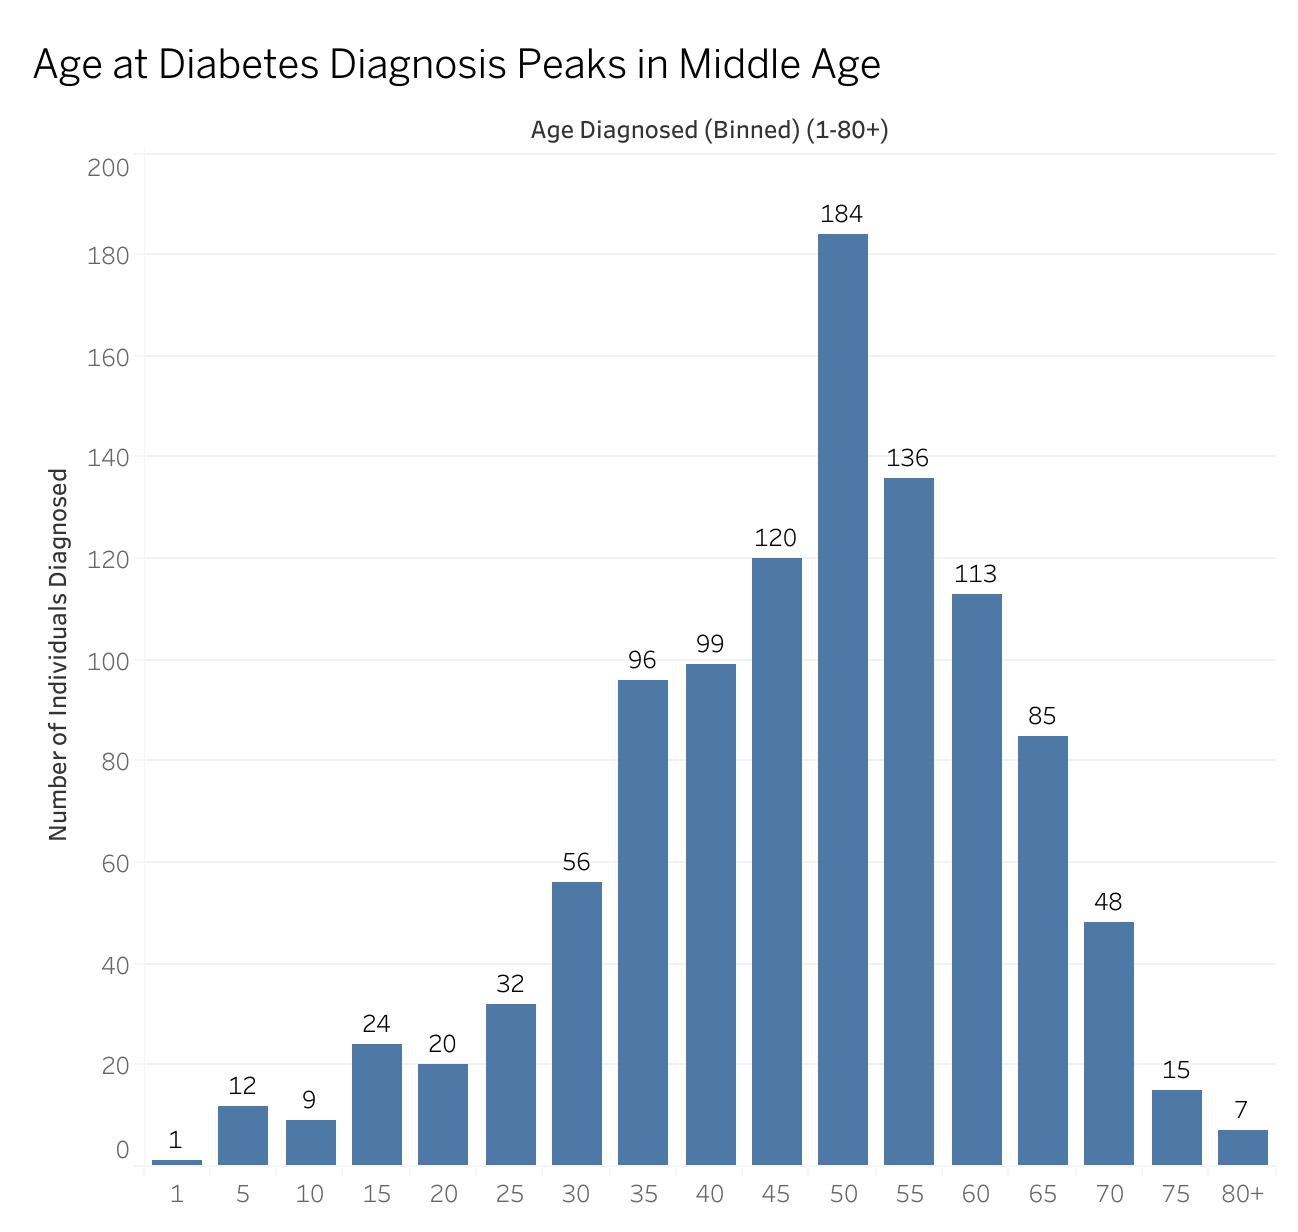
\includegraphics[width=0.8\linewidth]{../figures/Age Distribution of Diabetes Diagnoses} 

}

\caption{The age at which individuals reported being diagnosed with diabetes. Diagnoses begin in the mid-twenties, increase steadily, and peak between ages 50-55. These findings emphasize the importance of early screening and intervention before middle age to prevent and manage diabetes more effectively.}\label{fig:fig_age_diagnosis_distribution}
\end{figure}

The next figure shows that individuals show signs of borderline diabetes
and prediabetes starting in late teen years and early twenties.

\begin{figure}[H]

{\centering 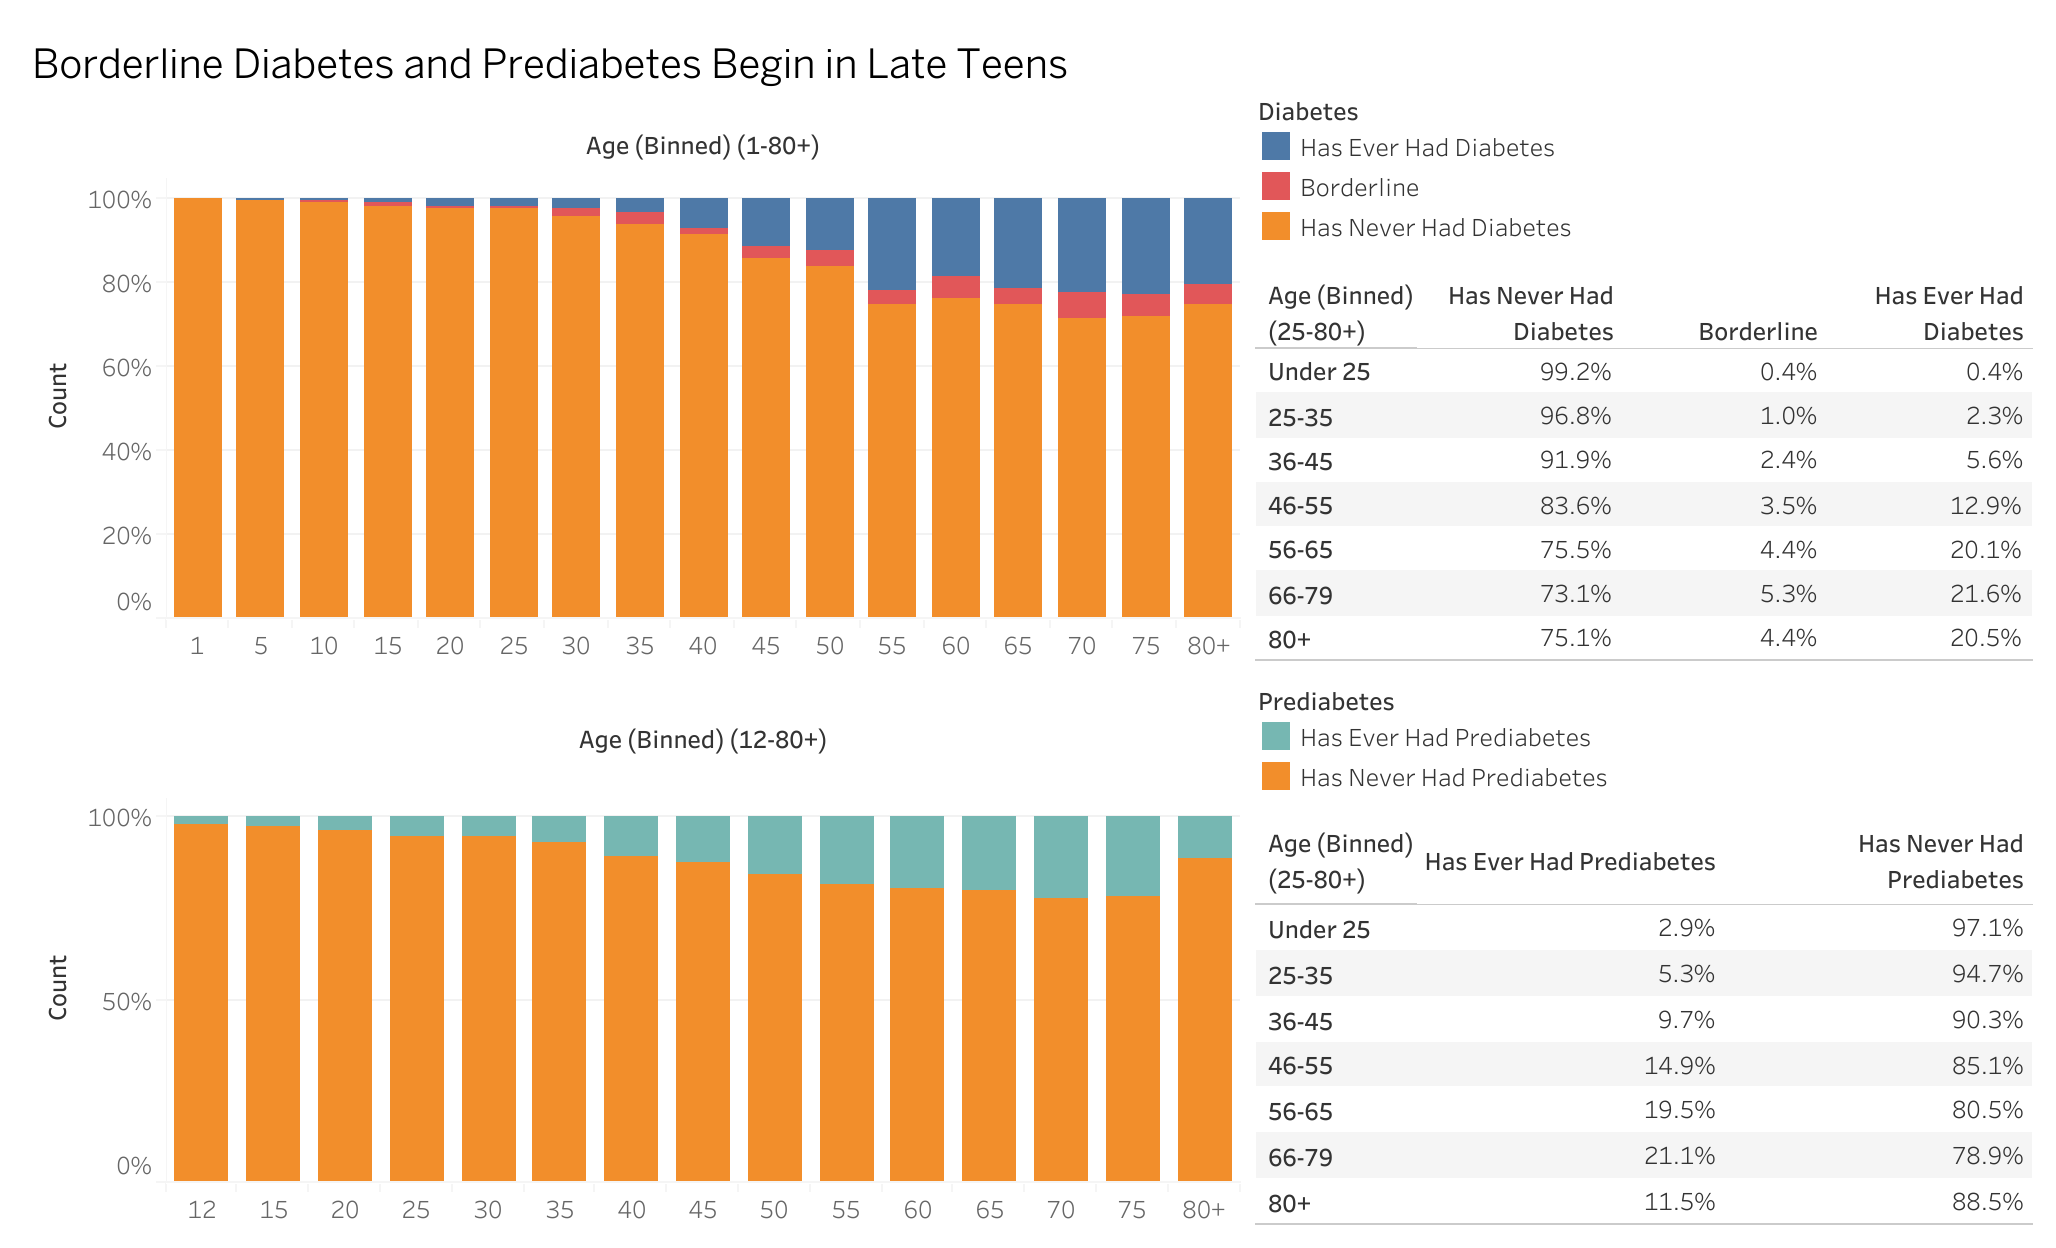
\includegraphics[width=0.9\linewidth]{../figures/Early Indicators of Diabetes Risk in Adolescents And Young Adults} 

}

\caption{Signs of borderline diabetes and prediabetes begin in the late teens and early twenties. Since prediabetes precedes Type 2 Diabetes, screening and lifestyle interventions should be prioritized for younger populations to mitigate future risks.}\label{fig:fig_prediabetes_indicators}
\end{figure}

Based on these findings further analysis focuses on young adults and
middle-aged groups to explore disparities in greater depth. Key findings
reveal that younger adults, individuals with lower income, and those
without health insurance are significantly less likely to undergo blood
testing for diabetes. Additionally, gender disparities and hypertension
are strongly associated with diabetes risk. Below, we examine each of
these findings in detail.

Younger adults are the least likely to get tested. Potential reasons
include financial constraints, lack of awareness, and limited healthcare
access. This disparity suggests a need for targeted outreach programs
focused on younger demographics. The rest of this analysis excludes the
older group to further look at the lack of testing for the rest of these
individuals.

\begin{figure}[H]

{\centering 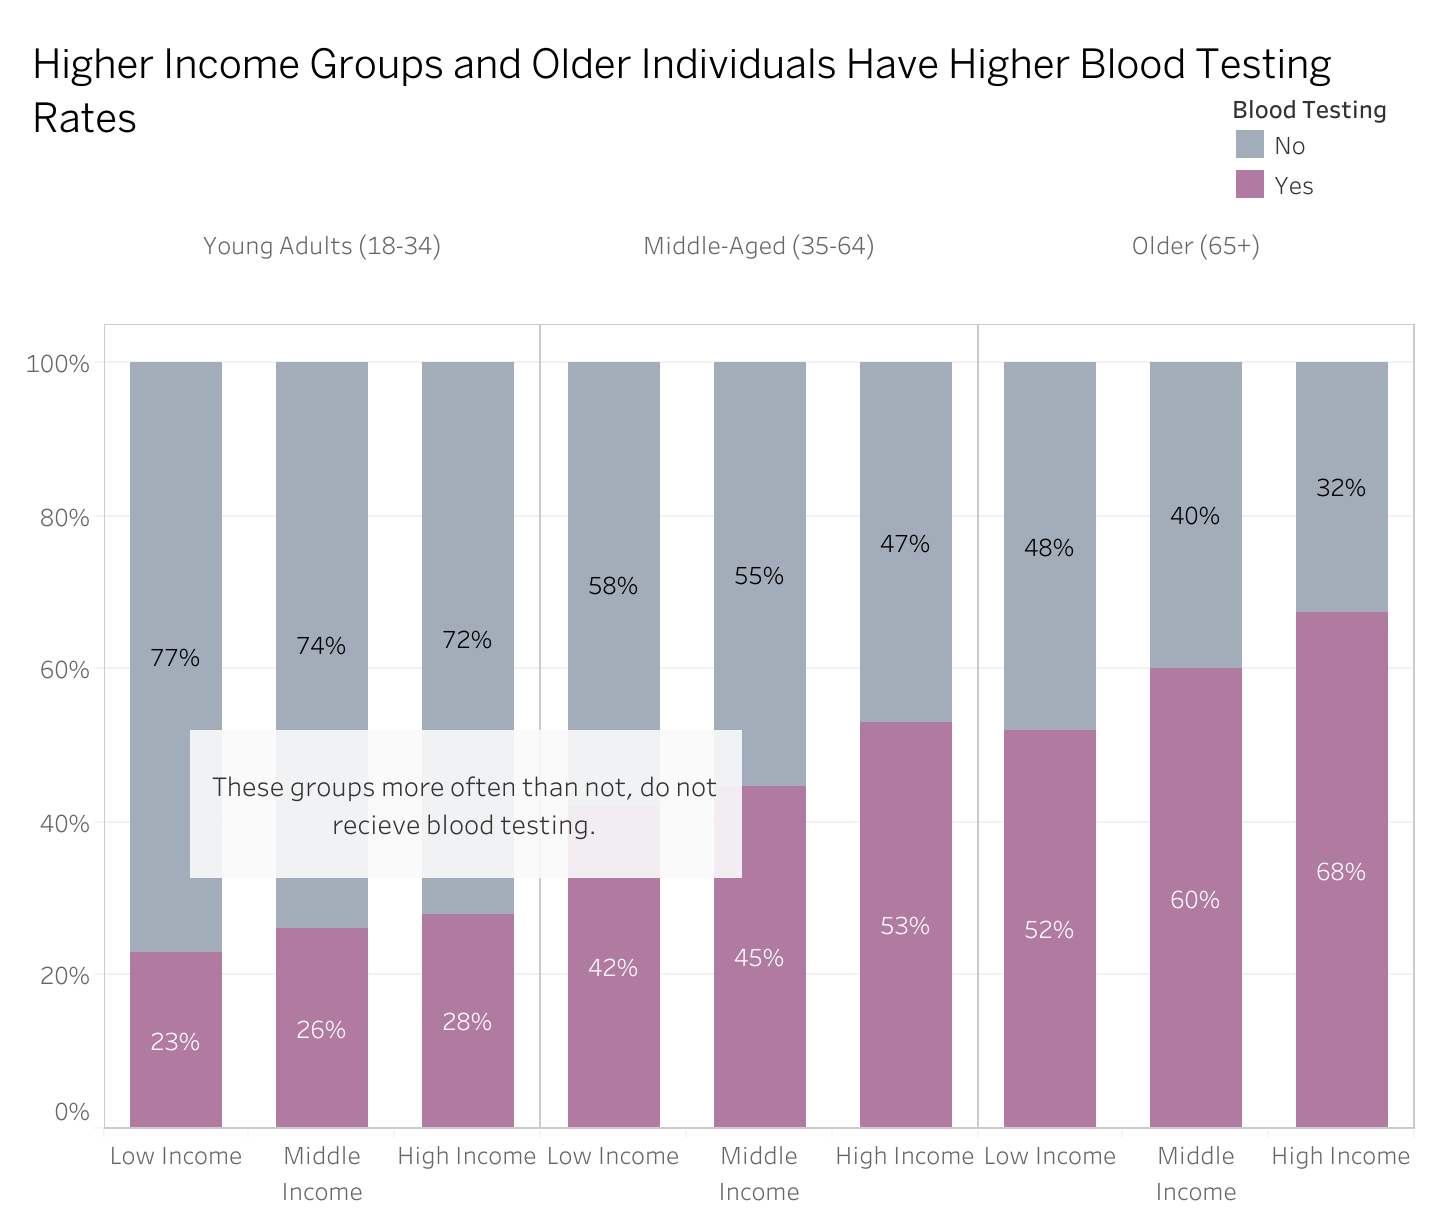
\includegraphics[width=0.7\linewidth]{../figures/Blood Testing Disparities by Age and Income} 

}

\caption{This visual demonstrates that younger adults and lower-income individuals have significantly lower blood testing rates, suggesting key barriers to healthcare access in these groups. Young Adults (18-34) are 62.7\% less likely to test than Middle-Aged Adults (OR = 0.373, 95\% CI: [0.324, 0.427], p < 1.25e-44). Low-Income individuals are 32.2\% less likely to test than High-Income (OR = 0.678, 95\% CI: [0.585 , 0.786], p < 2.81e-7). Middle-Income individuals are 22.4\% less likely to test than High-Income individuals (OR = 0.776, 95\% CI: [0.637, 0.944], p = 1.15e-2). These findings highlight critical disparities in access to preventive care.}\label{fig:fig_testing_by_age_income}
\end{figure}

Several factors influence blood testing rates. Health insurance plays a
vital role in diabetes testing. Individuals without health insurance are
less likely to undergo testing, emphasizing the role of expanding
healthcare coverage and promoting free or low-cost testing programs.
Insured young adults often do not undergo testing. While access to
healthcare insurance improves access, other factors can also play a role
such as inconsistent healthcare visits, lack of physician
recommendations, or a limited awareness contributes to lowered testing
rates. This suggests education and a more proactive engagement with a
physician are necessary elements to include, alongside healthcare
coverage. Education level influences testing behavior such that
individuals with a higher education correlate to higher rates of
testing. Health literacy influences health care behaviors suggesting the
need to target lower-education individuals.

\begin{figure}[H]

{\centering 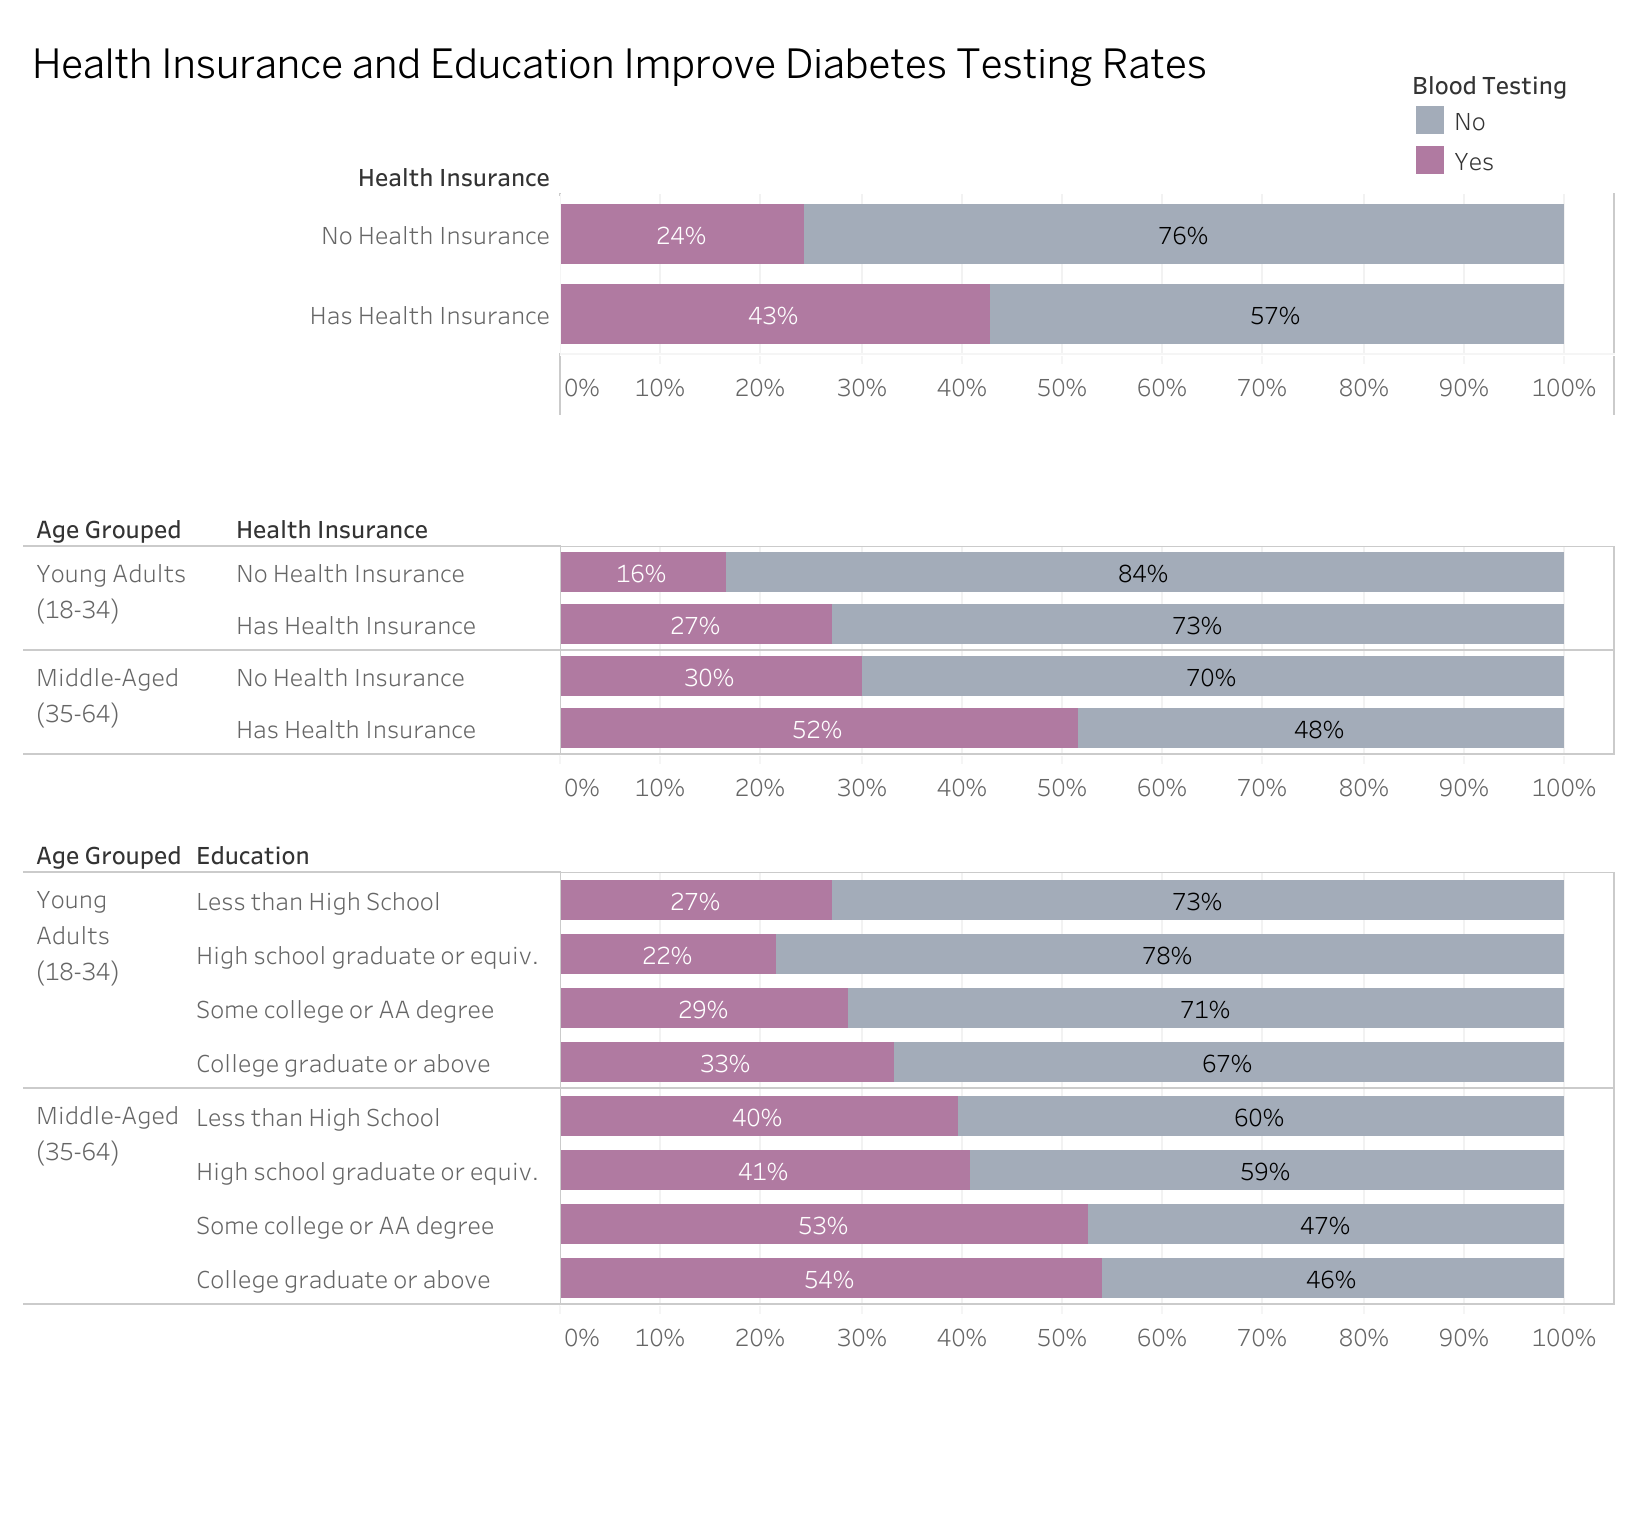
\includegraphics[width=0.8\linewidth]{../figures/Health Insurance and Education in Blood Testing} 

}

\caption{Health insurance significantly increases diabetes testing rates. Insured individuals are 76\% more likely to test than uninsured individuals (RR = 1.76, 95\% CI: [1.52, 2.03], p < 2.22e-16). Young Adults are 64\% less likely to test than Middle-Aged Adults (OR = 0.360, 95\% CI: [0.316, 0.409], p < 7.10e-55). Individuals with health insurance are 127\% more likely to get tested compared to uninsured individuals (OR = 2.27, 95\% CI: [1.87, 2.78], p < 3.92e-16). College Graduates are 68\% more likely to get tested compared to those with less than a high school education (OR = 1.68, 95\% CI: [1.37, 2.07], p < 1.03e- 6). Some College/AA Degree individuals are 52\% more likely to test than those with less than a high school education (OR = 1.52, 95\% CI: [1.23, 1.88], p < 1.13e-4). High school graduates do not test significantly more than those with less than a high school education (p = 0.807). These results reinforce the importance of expanding healthcare coverage and health literacy programs.}\label{fig:fig_testing_by_insurance_education}
\end{figure}

While socioeconomic factors strongly influence testing rates, gender
disparities also play a critical role. Gender disparities in testing
rates are strongly evident in younger adults. Specifically, young men
are 38.9\% less likely to undergo blood testing than young women,
indicating a need for gender-targeted awareness campaigns.

\begin{figure}[H]

{\centering 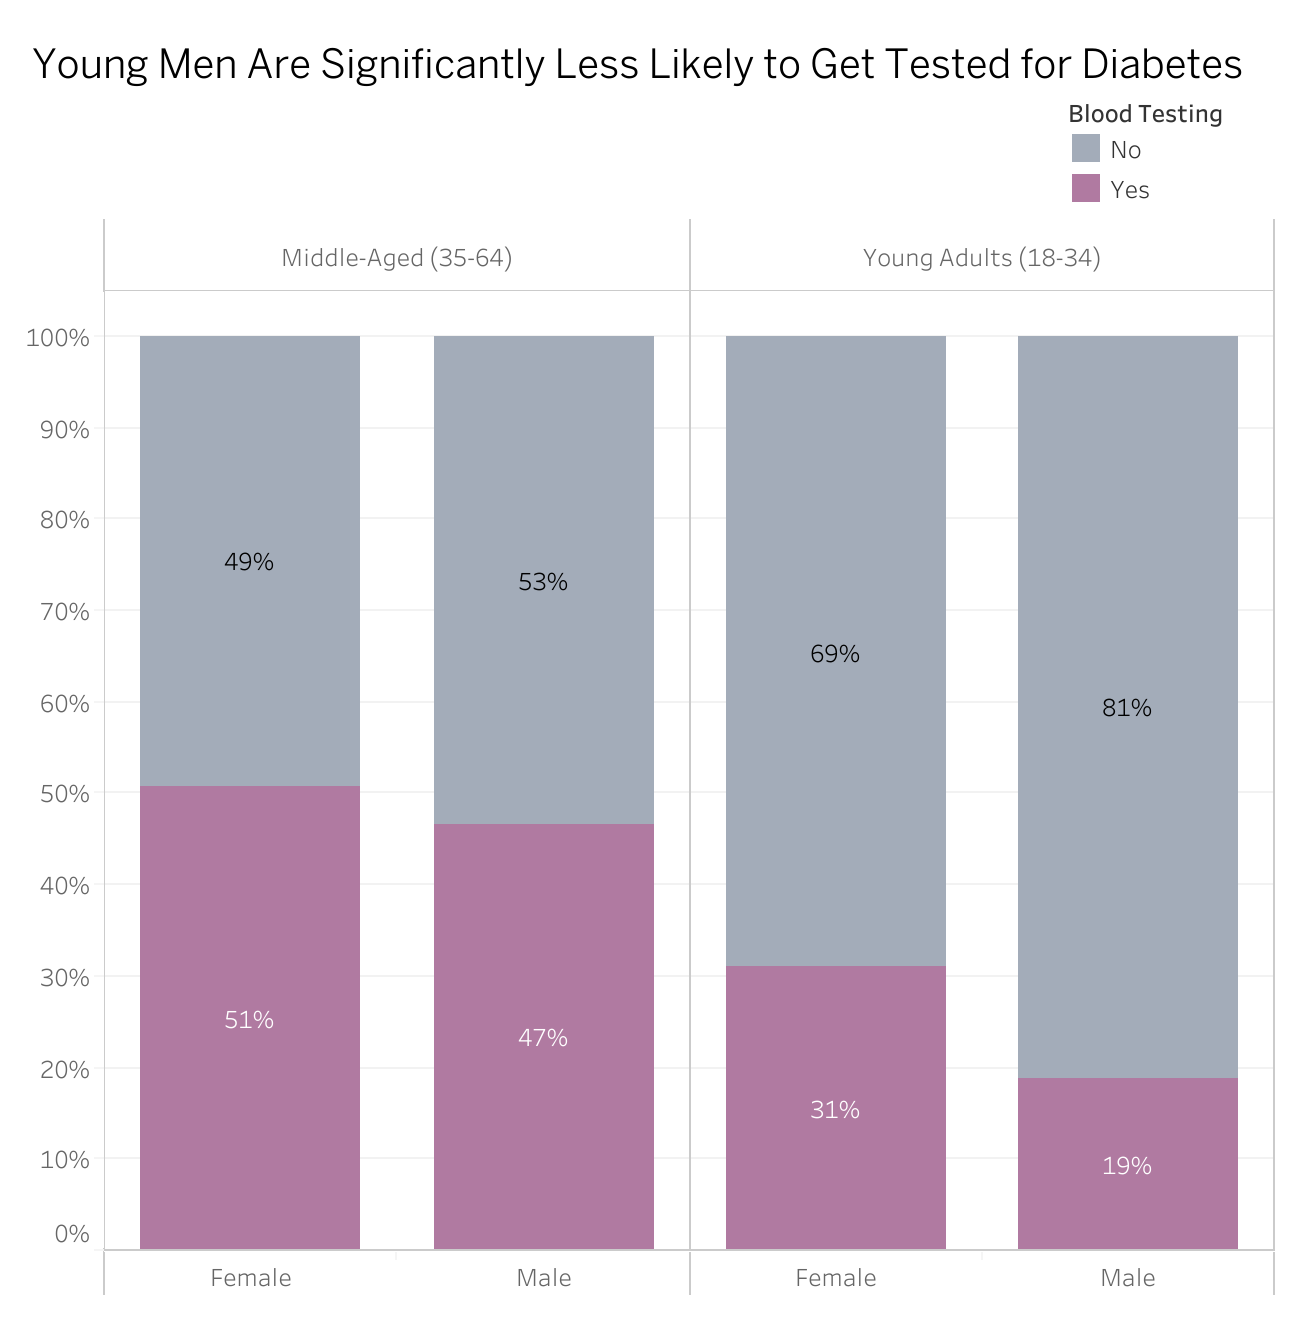
\includegraphics[width=0.6\linewidth]{../figures/Gender Disparities in Diabetes Testing} 

}

\caption{A disparity in blood testing rates across gender is shown here, where young men are significantly less likely to be tested than women, emphasizing the need for targeted outreach to this demographic. Among Young Adults, Males are 38.9\% less likely to undergo blood testing than Females (OR = 0.611, 95\% CI: [0.469, 0.794], p < 2.42e-4). These findings suggest the need for gender-specific awareness campaigns encouraging early diabetes screening in men.}\label{fig:fig_gender_testing_disparity}
\end{figure}

In addition to demographic disparities, we find strong associations
between hypertension and diabetes, highlighting another crucial risk
factor.

\begin{figure}[H]

{\centering 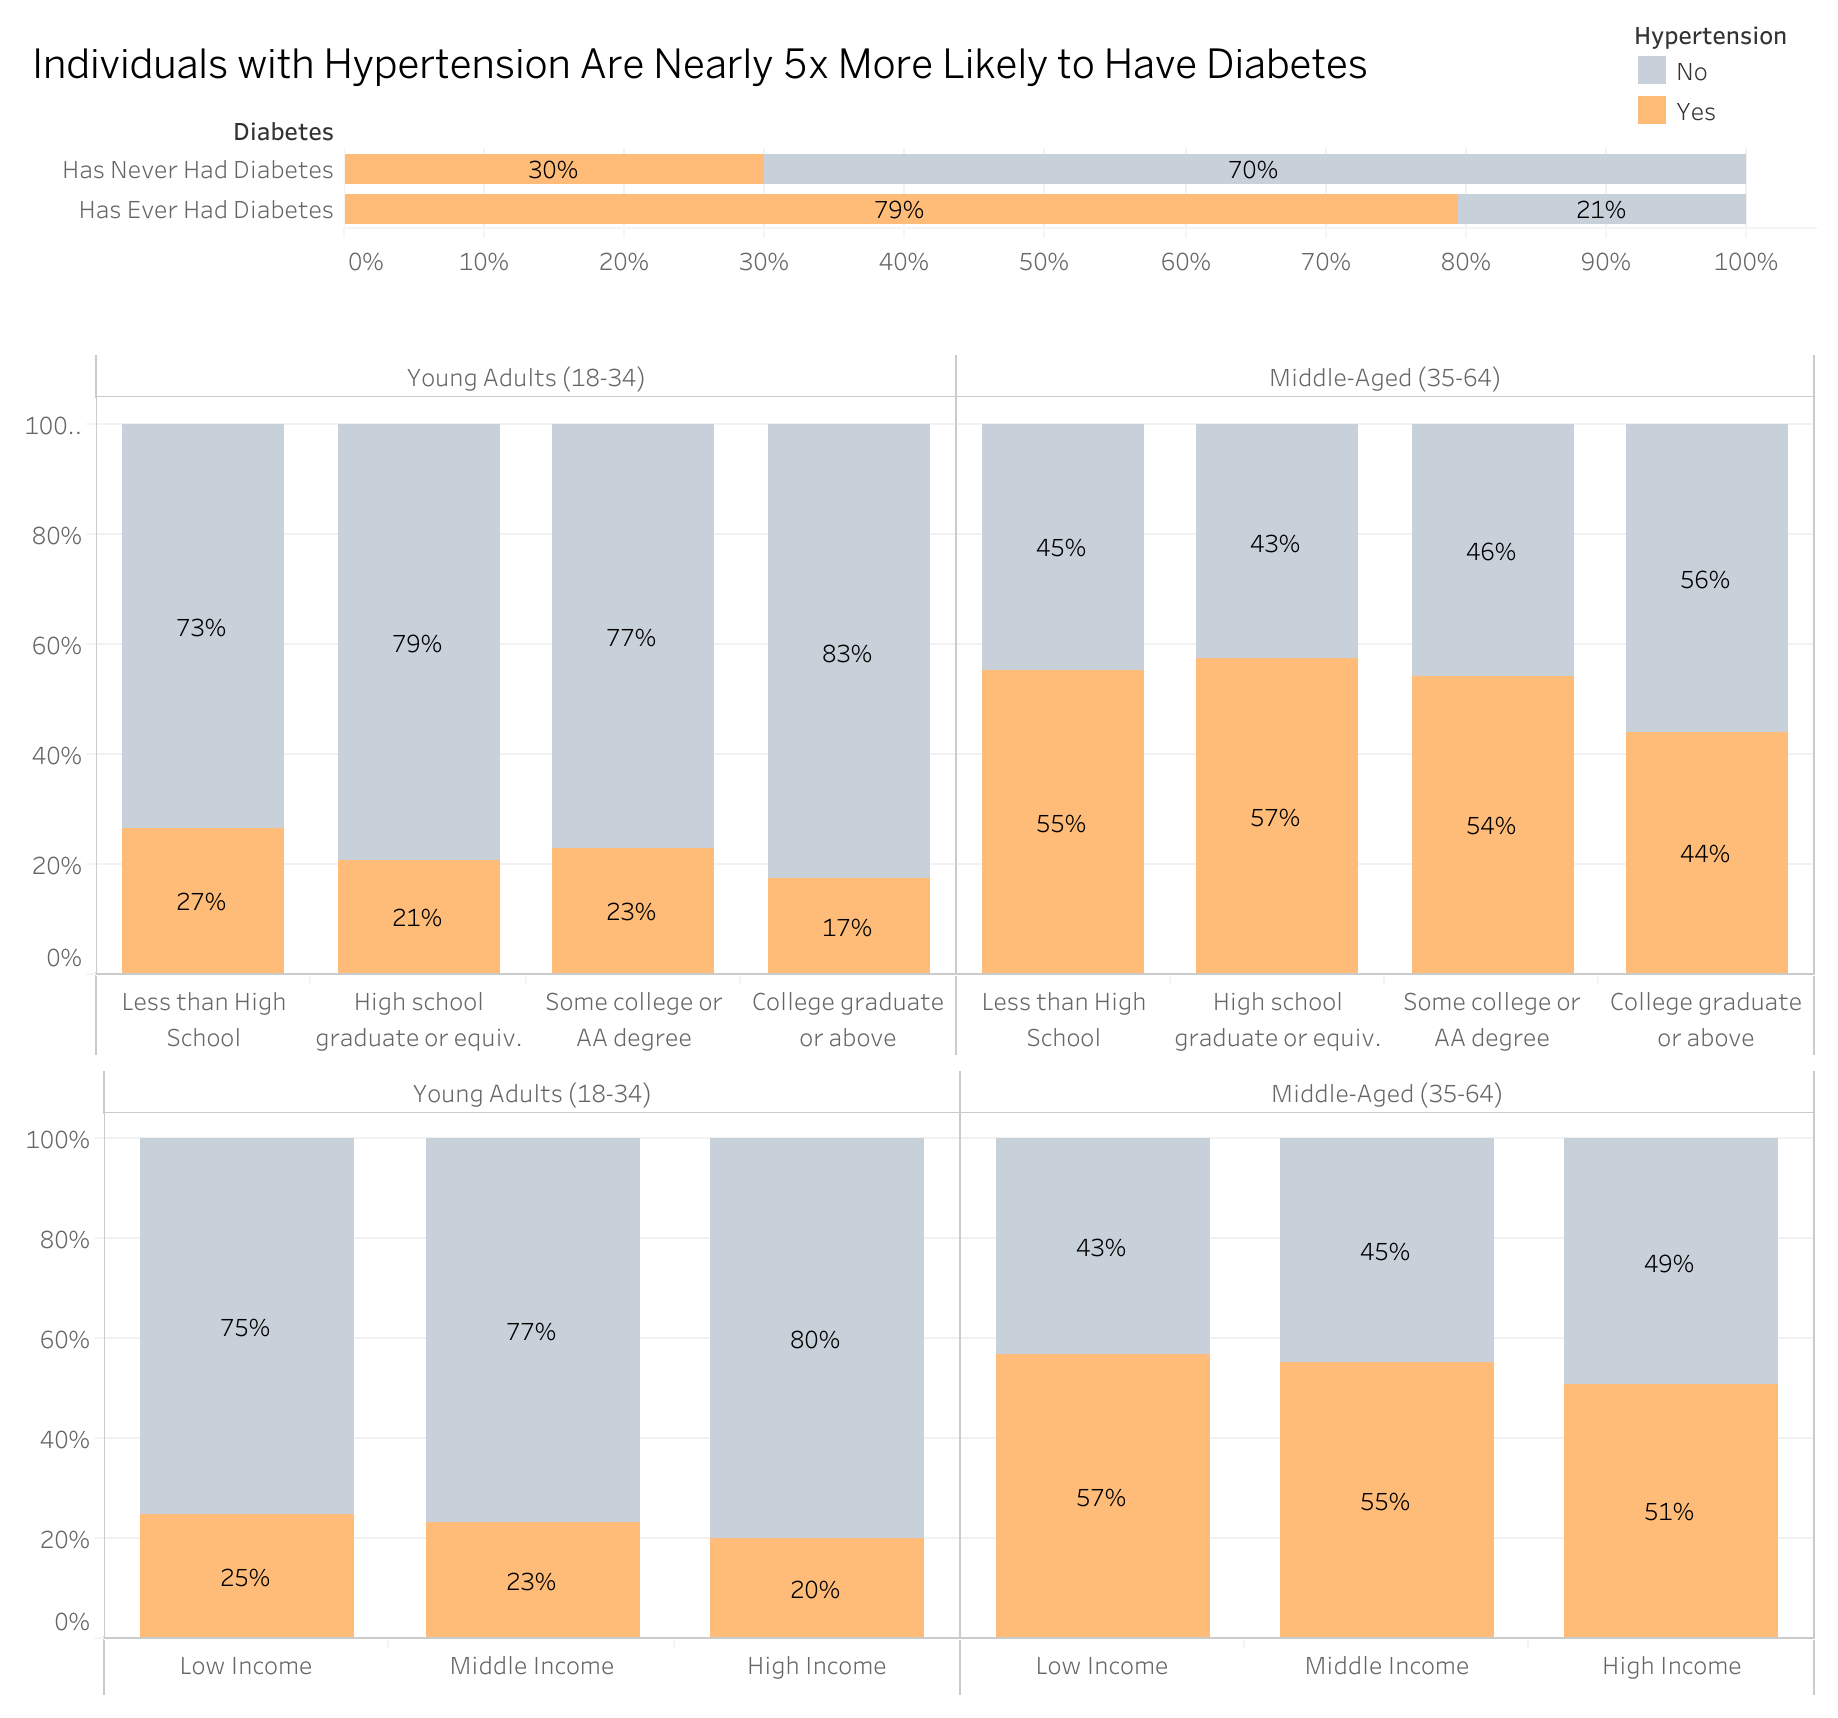
\includegraphics[width=0.8\linewidth]{../figures/Link Between Hypertension and Diabetes} 

}

\caption{Hypertensive individuals are nearly 4.98 times more likely to have Diabetes than those without Hypertension (RR = 4.98, 95\% CI: [4.08, 6.07], p < 2.22e-16). College Graduates are 37.4\% less likely to have Hypertension than those with less than a High School education (OR = 0.626, 95\% CI: [0.518, 0.757], p < 1.32e- 6). Low-Income individuals are 27\% more likely to have Hypertension than High-Income individuals (OR = 1.27, 95\% CI: [1.10, 1.46], p = 0.0008). These results suggest that managing hypertension could be an important strategy in preventing diabetes.}\label{fig:fig_hypertension_diabetes}
\end{figure}

These findings reinforce the importance of targeted interventions,
policy changes, and educational outreach to address disparities in
diabetes testing and prevention. Future studies should explore
additional behavioral and systemic barriers that may further contribute
to these trends.

\section{Implications and
Recommendations}\label{implications-and-recommendations}

With these finding, the follow recommendations can be given:

\begin{itemize}
\item
  There is a need for increased public outreach and awareness. Young
  adults and lower income individuals need targeted health campaigns
  emphasizing the importance of early testing. Modern tools such as
  social media, mobile health apps, and digital healthcare platforms can
  effectively reach younger populations and improve engagement.
\item
  Expand access to preventative care and community-based testing
  programs: Low-income communities should have access to free or
  reduced-cost screenings, particularly for uninsured individuals.
  Mobile clinics and community health programs can help bridge
  healthcare access gaps.
\item
  Enhance access to primary care providers and telehealth services: Many
  young adults and low-income individuals may lack a regular primary
  care provider. Telehealth platforms should be expanded to facilitate
  virtual consultations and provide convenient options for ordering
  blood tests at nearby clinics or hospitals.
\end{itemize}

\section{Interactive Dashboard}\label{interactive-dashboard}

To explore the data interactively, visit the Tableau dashboard:\\
\href{https://public.tableau.com/app/profile/jesus.torres.carbajal/viz/Diabetes_Case_Study/AgeDistributionofDiabetesDiagnoses?publish=yes}{Interactive
Tableau Dashboard -- Diabetes Case Study}

\section{Limitations and Future Work}\label{limitations-and-future-work}

While this analysis provides valuable insights into disparities in
diabetes screening, several limitations must be acknowledged. The NHANES
dataset relies on self-reported responses, which may introduce recall
bias and affect data accuracy. Additionally, selection bias exists as
higher income individuals are over represented compared to lower-income
groups, potentially limiting the generalization of these findings. The
sample size also restricted deeper racial and ethnic subgroup analyses,
making it difficult to assess disparities in underrepresented
populations. Furthermore, missing data required filtering, reducing the
dataset size and possibly influencing statistical significance. Finally,
as a cross-sectional dataset, NHANES captures data at a single point in
time, preventing the establishment of causal relationships or tracking
trends over time. Future research should focus on longitudinal studies,
expanding data collection efforts to include diverse racial, ethnic, and
socioeconomic groups, and developing targeted interventions to improve
healthcare accessibility and address systemic disparities in diabetes
prevention and diagnosis.

\section{Appendix A : Full Data Cleaning
Code}\label{appendix-a-full-data-cleaning-code}

This appendix provides a complete overview of the data collection and
preprocessing steps used in this analysis. The data was obtained from
NHANES, cleaned, and transformed for consistency and usability. Below
are the key steps involved.

\begin{itemize}
\tightlist
\item
  Automated Data Collection: Scrape NHANES \texttt{.xpt} files directly
  from the CDC website using \texttt{rvest}. Download and store these
  files in a structured format.
\item
  Merging and Cleaning: Merged demographic, health, and laboratory
  datasets based on unique IDs (SEQN). Re-coded categorical variables
  for better readability according to NHANES documentation. Created age
  groups, BMI categories, and hypertension indicators.
\item
  Handling Missing Data: Retained as much valid data as possible while
  filtering incomplete values. Standardized income, education, and
  health insurance fields for individuals who lacked a response for
  every field.
\end{itemize}

\subsection{Load Required Libraries}\label{load-required-libraries}

The following R packages are required to scrape, load, and clean the
NHANES dataset.

\begin{Shaded}
\begin{Highlighting}[]
\FunctionTok{library}\NormalTok{(rvest)        }\CommentTok{\# Web scraping to extract .xpt file URLS from the NHANES website }
\FunctionTok{library}\NormalTok{(haven)        }\CommentTok{\# Read .xpt files}
\FunctionTok{library}\NormalTok{(dplyr)        }\CommentTok{\# Data cleaning and transformation}
\end{Highlighting}
\end{Shaded}

\subsection{Automated Data Collection: Scraping and Importing NHANES
Data}\label{automated-data-collection-scraping-and-importing-nhanes-data}

The NHANES dataset is spread across multiple \texttt{.xpt} files hosted
on the CDC website. The script below automates downloading and importing
these datasets. The steps taken are as follows:

\begin{itemize}
\tightlist
\item
  Define NHANES URLs for different data categories.
\item
  Extract links to \texttt{.xpt} files
\item
  Download the files into the raw data folder.
\item
  Read all files into R as a \texttt{tibble}.
\item
  Apply meaningful names as headers to this dataset.
\end{itemize}

\subsection{Cleaning and Transforming the NHANES
Dataset}\label{cleaning-and-transforming-the-nhanes-dataset}

Once imported, the data must be cleaned and formatted for usability. The
following steps were taken:

\begin{itemize}
\tightlist
\item
  Merged datasets based on SEQN, a unique identifier for each
  participant.
\item
  Re-coded categorical variables (e.g., education, gender, race) based
  on NHANES documentation.
\item
  Created grouped variables for:

  \begin{itemize}
  \tightlist
  \item
    Age Grouped: Split into categories representing youth (1--17), young
    adults (18--34), middle-aged adults (35--64), and older adults
    (65+).
  \item
    BMI Group: Categorized based on CDC cutoffs: underweight
    (\textless18.5), normal (18.5--24.9), overweight (25--29.9), and
    three classes of obesity (30+).
  \item
    Income: Grouped into low, middle, and high income based on the
    federal poverty index. Income categories were derived from the
    Monthly Poverty Level Index, where values ≤1.30 represent low
    income, 1.30--1.85 represent middle income, and values
    \textgreater1.85 represent higher income.
  \end{itemize}
\item
  Defined health-related factors:

  \begin{itemize}
  \tightlist
  \item
    Age Diagnosed: Self-reported age when a doctor or other health
    professional first told to have had diabetes or sugar diabetes
  \item
    Blood Testing: Defined as having had a blood test for diabetes
    within the past three years.
  \item
    Diabetes and Prediabetes: Based on self-reported diagnosis and
    follow-up questions.
  \item
    Hypertension: Defined as having high blood pressure if a participant
    (1) self-reports it, (2) takes medication for it, or (3) has average
    systolic ≥130 or diastolic ≥80 mmHg.
  \end{itemize}
\item
  Handled missing or unusable data using \texttt{NA} to ensure
  consistency and completeness across variables.
\end{itemize}

\section{Appendix B: Generating
Statistics}\label{appendix-b-generating-statistics}

\subsection{Preparing the Dataset for Statistical
Analysis}\label{preparing-the-dataset-for-statistical-analysis}

This section modifies the cleaned dataset to allow executing functions
for generating statistics to help draw the conclusions in the main
project above. Variables like Diabetes were transformed into binary form
to support statistical models such as Relative Risk analysis. Reference
levels were re-ordered to ensure clarity in regression models, setting
baseline categories for comparison, such as comparing other groups to
``Middle-Aged'' adults or ``High Income''. Younger Adults and
Middle-Aged Adults were found to play a significant role in this
analysis, and as such, the other age groups were excluded to allow for
more of a focus.

\begin{Shaded}
\begin{Highlighting}[]
\NormalTok{stat\_ready\_data }\OtherTok{\textless{}{-}}\NormalTok{ cleaned\_data }\SpecialCharTok{\%\textgreater{}\%}
  \FunctionTok{filter}\NormalTok{(}\SpecialCharTok{!}\NormalTok{(Age\_Grouped }\SpecialCharTok{\%in\%} \FunctionTok{c}\NormalTok{(}\StringTok{"Children \& Teens (1{-}17)"}\NormalTok{, }\StringTok{\textquotesingle{}Older (65+)\textquotesingle{}}\NormalTok{))) }\SpecialCharTok{\%\textgreater{}\%} 
  \FunctionTok{mutate}\NormalTok{(}\AttributeTok{DiabetesBinary =} \FunctionTok{factor}\NormalTok{(}\FunctionTok{case\_when}\NormalTok{(}
\NormalTok{    Diabetes }\SpecialCharTok{==} \StringTok{"Has Diabetes"} \SpecialCharTok{\textasciitilde{}} \StringTok{"Yes"}\NormalTok{,}
    \ConstantTok{TRUE} \SpecialCharTok{\textasciitilde{}} \StringTok{"No"}
\NormalTok{  )),}
  \AttributeTok{Age\_Grouped =} \FunctionTok{droplevels}\NormalTok{(Age\_Grouped),}
  \AttributeTok{Age\_Grouped =} \FunctionTok{fct\_relevel}\NormalTok{(Age\_Grouped, }\StringTok{"Middle{-}Aged (35{-}64)"}\NormalTok{),}
  \AttributeTok{Blood\_Testing =} \FunctionTok{fct\_relevel}\NormalTok{(Blood\_Testing, }\StringTok{\textquotesingle{}No\textquotesingle{}}\NormalTok{),}
  \AttributeTok{BMI\_Group =} \FunctionTok{fct\_relevel}\NormalTok{(BMI\_Group, }\StringTok{"Normal Weight"}\NormalTok{),}
  \AttributeTok{Education =} \FunctionTok{fct\_relevel}\NormalTok{(Education, }\StringTok{"Less than High School"}\NormalTok{),}
  \AttributeTok{Gender =} \FunctionTok{fct\_relevel}\NormalTok{(Gender, }\StringTok{"Female"}\NormalTok{),}
  \AttributeTok{Health\_Insurance =} \FunctionTok{fct\_relevel}\NormalTok{(Health\_Insurance, }\StringTok{"No Health Insurance"}\NormalTok{),}
  \AttributeTok{Hypertension =} \FunctionTok{fct\_relevel}\NormalTok{(Hypertension, }\StringTok{"No"}\NormalTok{),}
  \AttributeTok{Income =} \FunctionTok{fct\_relevel}\NormalTok{(Income, }\StringTok{"High Income"}\NormalTok{),}
  \AttributeTok{Race =} \FunctionTok{fct\_relevel}\NormalTok{(Race, }\StringTok{"Non{-}Hispanic White"}\NormalTok{)}
\NormalTok{  )}

\FunctionTok{write.csv}\NormalTok{(stat\_ready\_data, }\StringTok{"../data/processed/stat\_ready\_data\_aug\_2021\_aug\_2023.csv"}\NormalTok{, }\AttributeTok{row.names =} \ConstantTok{FALSE}\NormalTok{)}
\end{Highlighting}
\end{Shaded}

\subsection{Statistical Methods}\label{statistical-methods}

\subsubsection{Chi-Square Test, Cramér's V, And Relative Risk
Analysis}\label{chi-square-test-cramuxe9rs-v-and-relative-risk-analysis}

This method uses a chi-square test to assess association between two
categorical variables, then calculates Cramér's V (effect size) and
Relative Risk (magnitude of risk associated with exposure).

\begin{Shaded}
\begin{Highlighting}[]
\CommentTok{\# Function to compute chi{-}square, Cramér’s V, and relative risk}
\NormalTok{generate\_relative\_risk }\OtherTok{\textless{}{-}} \ControlFlowTok{function}\NormalTok{(data, var1, var2, }\AttributeTok{remove\_na =} \ConstantTok{TRUE}\NormalTok{) \{}
  
  \CommentTok{\# Remove NAs from columns}
  \ControlFlowTok{if}\NormalTok{ (remove\_na) \{}
\NormalTok{    data }\OtherTok{\textless{}{-}}\NormalTok{ data }\SpecialCharTok{\%\textgreater{}\%} 
      \FunctionTok{filter}\NormalTok{(}\SpecialCharTok{!}\FunctionTok{is.na}\NormalTok{(data[[var1]]), }\SpecialCharTok{!}\FunctionTok{is.na}\NormalTok{(data[[var2]]))}
\NormalTok{  \}}
  
\NormalTok{  contingency\_table }\OtherTok{\textless{}{-}} \FunctionTok{table}\NormalTok{(data[[var1]], data[[var2]])}
  
  \CommentTok{\# Compute Chi{-}Square Test \& Cramér\textquotesingle{}s V}
\NormalTok{  stats }\OtherTok{\textless{}{-}} \FunctionTok{assocstats}\NormalTok{(contingency\_table)}
\NormalTok{  chi\_test }\OtherTok{\textless{}{-}}\NormalTok{ stats}\SpecialCharTok{$}\NormalTok{chisq\_tests[}\DecValTok{1}\NormalTok{, }\StringTok{"X\^{}2"}\NormalTok{]}
\NormalTok{  cramers\_v }\OtherTok{\textless{}{-}}\NormalTok{ stats}\SpecialCharTok{$}\NormalTok{cramer}
\NormalTok{  p\_value }\OtherTok{\textless{}{-}}\NormalTok{ stats}\SpecialCharTok{$}\NormalTok{chisq\_tests[}\DecValTok{1}\NormalTok{, }\StringTok{"P(\textgreater{} X\^{}2)"}\NormalTok{]}
  
  \CommentTok{\# Compute Relative Risk}
\NormalTok{  relative\_risk }\OtherTok{\textless{}{-}} \FunctionTok{riskratio}\NormalTok{(contingency\_table)}
  
\NormalTok{  results }\OtherTok{\textless{}{-}} \FunctionTok{tibble}\NormalTok{(}
    \AttributeTok{Statistic =} \FunctionTok{c}\NormalTok{(}\StringTok{"Chi{-}Square"}\NormalTok{, }\StringTok{"p{-}value"}\NormalTok{, }\StringTok{"Cramér\textquotesingle{}s V"}\NormalTok{, }\StringTok{"Relative Risk"}\NormalTok{,}
                  \StringTok{"Lower CI"}\NormalTok{, }\StringTok{"Upper CI"}\NormalTok{),}
    \AttributeTok{Value =} \FunctionTok{c}\NormalTok{(}
      \FunctionTok{signif}\NormalTok{(chi\_test, }\DecValTok{3}\NormalTok{),}
      \FunctionTok{format.pval}\NormalTok{(p\_value, }\AttributeTok{digits =} \DecValTok{3}\NormalTok{, }\AttributeTok{scientific =} \ConstantTok{TRUE}\NormalTok{),}
      \FunctionTok{signif}\NormalTok{(cramers\_v, }\DecValTok{3}\NormalTok{),}
      \FunctionTok{signif}\NormalTok{(relative\_risk}\SpecialCharTok{$}\NormalTok{measure[}\DecValTok{2}\NormalTok{,}\DecValTok{1}\NormalTok{], }\DecValTok{3}\NormalTok{),}
      \FunctionTok{signif}\NormalTok{(relative\_risk}\SpecialCharTok{$}\NormalTok{measure[}\DecValTok{2}\NormalTok{,}\DecValTok{2}\NormalTok{], }\DecValTok{3}\NormalTok{),}
      \FunctionTok{signif}\NormalTok{(relative\_risk}\SpecialCharTok{$}\NormalTok{measure[}\DecValTok{2}\NormalTok{,}\DecValTok{3}\NormalTok{], }\DecValTok{3}\NormalTok{)}
\NormalTok{      )}
\NormalTok{  )}
  
\NormalTok{  reference\_lvls }\OtherTok{\textless{}{-}} \FunctionTok{tibble}\NormalTok{(}
    \SpecialCharTok{!!}\AttributeTok{var1 :=} \FunctionTok{levels}\NormalTok{(data[[var1]])[}\DecValTok{1}\NormalTok{],}
    \SpecialCharTok{!!}\AttributeTok{var2 :=} \FunctionTok{levels}\NormalTok{(data[[var2]])[}\DecValTok{1}\NormalTok{])}
  
  \FunctionTok{return}\NormalTok{(}\FunctionTok{list}\NormalTok{(}\AttributeTok{Reference\_Levels =}\NormalTok{ reference\_lvls, }\AttributeTok{Results =}\NormalTok{ results))}
\NormalTok{\}}
\end{Highlighting}
\end{Shaded}

Example:

Relative Risk of Diabetes Testing Based on Health Insurance Status

\begin{longtable}[]{@{}cc@{}}
\caption{Baseline Categories for Categorical Variables.}\tabularnewline
\toprule\noalign{}
Health\_Insurance & Blood\_Testing \\
\midrule\noalign{}
\endfirsthead
\toprule\noalign{}
Health\_Insurance & Blood\_Testing \\
\midrule\noalign{}
\endhead
\bottomrule\noalign{}
\endlastfoot
No Health Insurance & No \\
\end{longtable}

\begin{longtable}[]{@{}cc@{}}
\caption{Summary Statistics and Relative Risk by Health Insurance
Status.}\tabularnewline
\toprule\noalign{}
Statistic & Value \\
\midrule\noalign{}
\endfirsthead
\toprule\noalign{}
Statistic & Value \\
\midrule\noalign{}
\endhead
\bottomrule\noalign{}
\endlastfoot
Chi-Square & 81.1 \\
p-value & \textless2e-16 \\
Cramér's V & 0.125 \\
Relative Risk & 1.76 \\
Lower CI & 1.53 \\
Upper CI & 2.03 \\
\end{longtable}

\subsubsection{Logistic Regression for Predicting Testing
Behavior}\label{logistic-regression-for-predicting-testing-behavior}

This function models how predictors such as age and income affect the
odds of undergoing blood testing or having a chronic condition like
hypertension.

\begin{Shaded}
\begin{Highlighting}[]
\CommentTok{\# Logistic regression modeling of an outcome variable based on two predictors, with an optional interaction term to explore combined effects.}
\NormalTok{generate\_logistic\_reg }\OtherTok{\textless{}{-}} \ControlFlowTok{function}\NormalTok{(data, outcome, var1, var2, }\AttributeTok{interaction =} \ConstantTok{TRUE}\NormalTok{, }\AttributeTok{remove\_na =} \ConstantTok{TRUE}\NormalTok{)\{}
  
  \CommentTok{\# Remove NAs from columns}
  \ControlFlowTok{if}\NormalTok{ (remove\_na) \{}
\NormalTok{    data }\OtherTok{\textless{}{-}}\NormalTok{ data }\SpecialCharTok{\%\textgreater{}\%} 
      \FunctionTok{filter}\NormalTok{(}\SpecialCharTok{!}\FunctionTok{is.na}\NormalTok{(data[[outcome]]), }\SpecialCharTok{!}\FunctionTok{is.na}\NormalTok{(data[[var1]]), }\SpecialCharTok{!}\FunctionTok{is.na}\NormalTok{(data[[var2]]))}
\NormalTok{  \}}
  
\NormalTok{  formula }\OtherTok{\textless{}{-}} \ControlFlowTok{if}\NormalTok{ (interaction) \{}
    \FunctionTok{paste0}\NormalTok{(outcome, }\StringTok{" \textasciitilde{} "}\NormalTok{, var1, }\StringTok{" * "}\NormalTok{, var2) }\CommentTok{\# Includes Interaction}
\NormalTok{  \} }\ControlFlowTok{else}\NormalTok{ \{}
    \FunctionTok{paste0}\NormalTok{(outcome, }\StringTok{" \textasciitilde{} "}\NormalTok{, var1, }\StringTok{" + "}\NormalTok{, var2) }\CommentTok{\# No interaction}
\NormalTok{  \}}
  
\NormalTok{  logistic\_reg }\OtherTok{\textless{}{-}} \FunctionTok{glm}\NormalTok{(}\FunctionTok{as.formula}\NormalTok{(formula), }\AttributeTok{data =}\NormalTok{ data, }\AttributeTok{family =}\NormalTok{ binomial)}
  
\NormalTok{  odds\_ratios }\OtherTok{\textless{}{-}} \FunctionTok{exp}\NormalTok{(}\FunctionTok{coef}\NormalTok{(logistic\_reg))}
\NormalTok{  conf\_intervals }\OtherTok{\textless{}{-}} \FunctionTok{exp}\NormalTok{(}\FunctionTok{confint}\NormalTok{(logistic\_reg))}
  
\NormalTok{  results }\OtherTok{\textless{}{-}} \FunctionTok{tibble}\NormalTok{(}
    \AttributeTok{Predictor =} \FunctionTok{names}\NormalTok{(odds\_ratios),}
    \AttributeTok{Odds\_Ratio =} \FunctionTok{signif}\NormalTok{(}\FunctionTok{as.numeric}\NormalTok{(odds\_ratios), }\DecValTok{3}\NormalTok{),}
    \AttributeTok{Lower\_CI =} \FunctionTok{signif}\NormalTok{(}\FunctionTok{as.numeric}\NormalTok{(conf\_intervals[, }\DecValTok{1}\NormalTok{]), }\DecValTok{3}\NormalTok{),}
    \AttributeTok{Upper\_CI =} \FunctionTok{signif}\NormalTok{(}\FunctionTok{as.numeric}\NormalTok{(conf\_intervals[, }\DecValTok{2}\NormalTok{]), }\DecValTok{3}\NormalTok{),}
    \AttributeTok{p\_value =} \FunctionTok{format.pval}\NormalTok{(}\FunctionTok{coef}\NormalTok{(}\FunctionTok{summary}\NormalTok{(logistic\_reg))[, }\DecValTok{4}\NormalTok{], }\AttributeTok{digits =} \DecValTok{3}\NormalTok{, }\AttributeTok{scientific =} \ConstantTok{TRUE}\NormalTok{)}
\NormalTok{  )}
  
\NormalTok{  reference\_lvls }\OtherTok{\textless{}{-}} \FunctionTok{tibble}\NormalTok{(}
    \SpecialCharTok{!!}\AttributeTok{outcome :=} \FunctionTok{levels}\NormalTok{(data[[outcome]])[}\DecValTok{1}\NormalTok{],}
    \SpecialCharTok{!!}\AttributeTok{var1 :=} \FunctionTok{levels}\NormalTok{(data[[var1]])[}\DecValTok{1}\NormalTok{],}
    \SpecialCharTok{!!}\AttributeTok{var2 :=} \FunctionTok{levels}\NormalTok{(data[[var2]])[}\DecValTok{1}\NormalTok{])}
  
  \FunctionTok{return}\NormalTok{(}\FunctionTok{list}\NormalTok{(}\AttributeTok{reference\_lvls =}\NormalTok{ reference\_lvls, }\AttributeTok{results =}\NormalTok{ results))}
\NormalTok{\}}
\end{Highlighting}
\end{Shaded}

Example:

Predicts Blood Testing based on Age Group and Income. Does not include
interaction effects.

\begin{longtable}[]{@{}ccc@{}}
\caption{Baseline Categories for Categorical Variables.}\tabularnewline
\toprule\noalign{}
Blood\_Testing & Age\_Grouped & Income \\
\midrule\noalign{}
\endfirsthead
\toprule\noalign{}
Blood\_Testing & Age\_Grouped & Income \\
\midrule\noalign{}
\endhead
\bottomrule\noalign{}
\endlastfoot
No & Middle-Aged (35-64) & High Income \\
\end{longtable}

\begin{longtable}[]{@{}
  >{\centering\arraybackslash}p{(\columnwidth - 8\tabcolsep) * \real{0.4400}}
  >{\centering\arraybackslash}p{(\columnwidth - 8\tabcolsep) * \real{0.1600}}
  >{\centering\arraybackslash}p{(\columnwidth - 8\tabcolsep) * \real{0.1333}}
  >{\centering\arraybackslash}p{(\columnwidth - 8\tabcolsep) * \real{0.1333}}
  >{\centering\arraybackslash}p{(\columnwidth - 8\tabcolsep) * \real{0.1333}}@{}}
\caption{Logistic Regression Results: Blood Testing. Odds Ratios with
95\% Confidence Intervals and p-values.}\tabularnewline
\toprule\noalign{}
\begin{minipage}[b]{\linewidth}\centering
Predictor
\end{minipage} & \begin{minipage}[b]{\linewidth}\centering
Odds\_Ratio
\end{minipage} & \begin{minipage}[b]{\linewidth}\centering
Lower\_CI
\end{minipage} & \begin{minipage}[b]{\linewidth}\centering
Upper\_CI
\end{minipage} & \begin{minipage}[b]{\linewidth}\centering
p\_value
\end{minipage} \\
\midrule\noalign{}
\endfirsthead
\toprule\noalign{}
\begin{minipage}[b]{\linewidth}\centering
Predictor
\end{minipage} & \begin{minipage}[b]{\linewidth}\centering
Odds\_Ratio
\end{minipage} & \begin{minipage}[b]{\linewidth}\centering
Lower\_CI
\end{minipage} & \begin{minipage}[b]{\linewidth}\centering
Upper\_CI
\end{minipage} & \begin{minipage}[b]{\linewidth}\centering
p\_value
\end{minipage} \\
\midrule\noalign{}
\endhead
\bottomrule\noalign{}
\endlastfoot
(Intercept) & 1.100 & 1.010 & 1.210 & 2.90e-02 \\
Age\_GroupedYoung Adults (18-34) & 0.373 & 0.324 & 0.427 & \textless{}
2e-16 \\
IncomeLow Income & 0.678 & 0.585 & 0.786 & 2.81e-07 \\
IncomeMiddle Income & 0.776 & 0.637 & 0.944 & 1.15e-02 \\
\end{longtable}

\section{Appendix C: Session
Information}\label{appendix-c-session-information}

\begin{verbatim}
## - Session info ---------------------------------------------------------------------------
##  setting  value
##  version  R version 4.4.2 (2024-10-31)
##  os       macOS Sequoia 15.3.2
##  system   aarch64, darwin20
##  ui       RStudio
##  language (EN)
##  collate  en_US.UTF-8
##  ctype    en_US.UTF-8
##  tz       America/Los_Angeles
##  date     2025-03-25
##  rstudio  2024.12.1+563 Kousa Dogwood (desktop)
##  pandoc   3.2 @ /Applications/RStudio.app/Contents/Resources/app/quarto/bin/tools/aarch64/ (via rmarkdown)
##  quarto   1.5.57 @ /Applications/RStudio.app/Contents/Resources/app/quarto/bin/quarto
## 
## - Packages -------------------------------------------------------------------------------
##  package     * version  date (UTC) lib source
##  bslib         0.9.0    2025-01-30 [1] CRAN (R 4.4.1)
##  cachem        1.1.0    2024-05-16 [1] CRAN (R 4.4.1)
##  cli           3.6.4    2025-02-13 [1] CRAN (R 4.4.1)
##  codetools     0.2-20   2024-03-31 [1] CRAN (R 4.4.2)
##  colorspace    2.1-1    2024-07-26 [1] CRAN (R 4.4.1)
##  curl          6.2.1    2025-02-19 [1] CRAN (R 4.4.1)
##  digest        0.6.37   2024-08-19 [1] CRAN (R 4.4.1)
##  dplyr       * 1.1.4    2023-11-17 [1] CRAN (R 4.4.0)
##  epitools    * 0.5-10.1 2020-03-22 [1] CRAN (R 4.4.1)
##  evaluate      1.0.3    2025-01-10 [1] CRAN (R 4.4.1)
##  fastmap       1.2.0    2024-05-15 [1] CRAN (R 4.4.1)
##  forcats     * 1.0.0    2023-01-29 [1] CRAN (R 4.4.0)
##  generics      0.1.3    2022-07-05 [1] CRAN (R 4.4.1)
##  glue          1.8.0    2024-09-30 [1] CRAN (R 4.4.1)
##  haven       * 2.5.4    2023-11-30 [1] CRAN (R 4.4.0)
##  here        * 1.0.1    2020-12-13 [1] CRAN (R 4.4.1)
##  hms           1.1.3    2023-03-21 [1] CRAN (R 4.4.0)
##  htmltools     0.5.8.1  2024-04-04 [1] CRAN (R 4.4.1)
##  httr          1.4.7    2023-08-15 [1] CRAN (R 4.4.0)
##  jquerylib     0.1.4    2021-04-26 [1] CRAN (R 4.4.0)
##  jsonlite      1.9.0    2025-02-19 [1] CRAN (R 4.4.1)
##  kableExtra  * 1.4.0    2024-01-24 [1] CRAN (R 4.4.0)
##  knitr       * 1.49     2024-11-08 [1] CRAN (R 4.4.1)
##  lattice       0.22-6   2024-03-20 [1] CRAN (R 4.4.2)
##  lifecycle     1.0.4    2023-11-07 [1] CRAN (R 4.4.1)
##  lmtest        0.9-40   2022-03-21 [1] CRAN (R 4.4.1)
##  magrittr      2.0.3    2022-03-30 [1] CRAN (R 4.4.1)
##  MASS          7.3-61   2024-06-13 [1] CRAN (R 4.4.2)
##  munsell       0.5.1    2024-04-01 [1] CRAN (R 4.4.1)
##  pillar        1.10.1   2025-01-07 [1] CRAN (R 4.4.1)
##  pkgconfig     2.0.3    2019-09-22 [1] CRAN (R 4.4.1)
##  R6            2.6.1    2025-02-15 [1] CRAN (R 4.4.1)
##  readr         2.1.5    2024-01-10 [1] CRAN (R 4.4.0)
##  rlang         1.1.5    2025-01-17 [1] CRAN (R 4.4.1)
##  rmarkdown   * 2.29     2024-11-04 [1] CRAN (R 4.4.1)
##  rprojroot     2.0.4    2023-11-05 [1] CRAN (R 4.4.1)
##  rstudioapi    0.17.1   2024-10-22 [1] CRAN (R 4.4.1)
##  rvest       * 1.0.4    2024-02-12 [1] CRAN (R 4.4.0)
##  sass          0.4.9    2024-03-15 [1] CRAN (R 4.4.0)
##  scales        1.3.0    2023-11-28 [1] CRAN (R 4.4.0)
##  selectr       0.4-2    2019-11-20 [1] CRAN (R 4.4.0)
##  sessioninfo   1.2.3    2025-02-05 [1] CRAN (R 4.4.1)
##  stringi       1.8.4    2024-05-06 [1] CRAN (R 4.4.1)
##  stringr       1.5.1    2023-11-14 [1] CRAN (R 4.4.0)
##  svglite       2.1.3    2023-12-08 [1] CRAN (R 4.4.0)
##  systemfonts   1.2.1    2025-01-20 [1] CRAN (R 4.4.1)
##  tibble        3.2.1    2023-03-20 [1] CRAN (R 4.4.0)
##  tidyselect    1.2.1    2024-03-11 [1] CRAN (R 4.4.0)
##  tzdb          0.4.0    2023-05-12 [1] CRAN (R 4.4.0)
##  vcd         * 1.4-13   2024-09-16 [1] CRAN (R 4.4.1)
##  vctrs         0.6.5    2023-12-01 [1] CRAN (R 4.4.0)
##  viridisLite   0.4.2    2023-05-02 [1] CRAN (R 4.4.1)
##  withr         3.0.2    2024-10-28 [1] CRAN (R 4.4.1)
##  xfun          0.51     2025-02-19 [1] CRAN (R 4.4.1)
##  xml2          1.3.7    2025-02-28 [1] CRAN (R 4.4.1)
##  yaml          2.3.10   2024-07-26 [1] CRAN (R 4.4.1)
##  zoo           1.8-13   2025-02-22 [1] CRAN (R 4.4.1)
## 
##  [1] /Library/Frameworks/R.framework/Versions/4.4-arm64/Resources/library
##  * -- Packages attached to the search path.
## 
## ------------------------------------------------------------------------------------------
\end{verbatim}

\section{References}\label{references}

Aragon T (2020). \emph{epitools: Epidemiology Tools}. R package version
0.5-10.1, \url{https://CRAN.R-project.org/package=epitools}.

Centers for Disease Control and Prevention (CDC). (2024). \emph{National
Health and Nutrition Examination Survey (NHANES)}. U.S. Department of
Health and Human Services. Retrieved from
\url{https://wwwn.cdc.gov/nchs/nhanes/}

Meyer D, Zeileis A, Hornik K, Friendly M (2024). \emph{vcd: Visualizing
Categorical Data}. R package version 1.4-13,
\url{https://CRAN.R-project.org/package=vcd}.

R Core Team (2024). \emph{R: A Language and Environment for Statistical
Computing}. R Foundation for Statistical Computing, Vienna, Austria.
\url{https://www.R-project.org/}.

Wickham H (2024). \emph{rvest: Easily Harvest (Scrape) Web Pages}. R
package version 1.0.4, \url{https://CRAN.R-project.org/package=rvest}.

Wickham H (2023). \emph{forcats: Tools for Working with Categorical
Variables (Factors)}. R package version 1.0.0,
\url{https://CRAN.R-project.org/package=forcats}.

Wickham H, François R, Henry L, Müller K, Vaughan D (2023). \emph{dplyr:
A Grammar of Data Manipulation}. R package version 1.1.4,
\url{https://CRAN.R-project.org/package=dplyr}.

Wickham H, Miller E, Smith D (2023). \emph{haven: Import and Export
`SPSS', `Stata' and `SAS' Files}. R package version 2.5.4,
\url{https://CRAN.R-project.org/package=haven}.

Xie Y (2024). \emph{knitr: A General-Purpose Package for Dynamic Report
Generation in R}. R package version 1.49,
\url{https://yihui.org/knitr/}.

Yihui Xie (2015) Dynamic Documents with R and knitr. 2nd edition.
Chapman and Hall/CRC. ISBN 978-1498716963

Yihui Xie (2014) knitr: A Comprehensive Tool for Reproducible Research
in R. In Victoria Stodden, Friedrich Leisch and Roger D. Peng, editors,
Implementing Reproducible Computational Research. Chapman and Hall/CRC.
ISBN 978-1466561595

\end{document}
